\documentclass{include/protokollclass}
% Main File - Based on protokollclass.cls
% Comments are mostly in English (and some in German, concerning the Praktikum)
% ------------------------------------------------------------------------------
% Further files in folder:
%  - include/cmds.tex (for macros and additional commands)
%  - include/kitlogo.pdf (for titlepage)
%  - lit.bib (bibtex bibliography database)
%  - include/titlepage.tex (for layout of titelpage)
% ------------------------------------------------------------------------------
% Useful Supplied Packages:
% amsmath, amssymb, mathtools, bbm, upgreek, nicefrac,
% siunitx, varioref, booktabs, graphicx, tikz, multicol





%% ---------------------------------------------
%% |    Informationen über dieses Protokoll    |
%% ---------------------------------------------
\newcommand{\praktikum}{P1}                % P1 oder P2
\newcommand{\semester}{WS19/20}            % z.B. "WS14/15" oder "SS15"

\newcommand{\wochentag}{Do}                % Mo, Di, Mi oder Do
\newcommand{\gruppennr}{15}                % Zweistellige Gruppennummer

\newcommand{\nachnamea}{Kraus}             % Nachname des ersten Praktikanten
\newcommand{\vornamea}{Steven}               % Vorname des ersten Praktikanten
\newcommand{\nachnameb}{Ries}              % Nachname des zweiten Praktikanten
\newcommand{\vornameb}{Niklas}              % Vorname des zweiten Praktikanten

\newcommand{\emailadressen}{}
% optionale Angabe von Emailadresse(n) für den Kontakt mit dem Betreuer

\newcommand{\versuch}{Kreisel} % Name des Versuchs
\newcommand{\versuchsnr}{71}               % bitte die korrekte Nummer dem 
                                           % Arbeitsplatz am Versuchstag 
                                           % entnehmen
\newcommand{\fehlerrechnung}{Nein}         % Ob Fehlerrechnung im Versuch 
                                           % durchgeführt wurde oder nicht

\newcommand{\betreuer}{}      % Name des zuständigen Betreuers
\newcommand{\durchgefuehrt}{24.10.19}      % Datum, an dem der Versuch 
                                           % durchgeführt wurde





%% --------------------------------------
%% |    Settings for Word Separation    |
%% --------------------------------------
% Help for separation:
% In German package the following hints are additionally available:
% "- = Additional separation
% "| = Suppress ligation and possible separation (e.g. Schaf"|fell)
% "~ = Hyphenation without separation (e.g. bergauf und "~ab)
% "= = Hyphenation with separation before and after
% "" = Separation without a hyphenation (e.g. und/""oder)

% Describe separation hints here:
\hyphenation
{
    über-nom-me-nen an-ge-ge-be-nen
    %Pro-to-koll-in-stan-zen
    %Ma-na-ge-ment  Netz-werk-ele-men-ten
    %Netz-werk Netz-werk-re-ser-vie-rung
    %Netz-werk-adap-ter Fein-ju-stier-ung
    %Da-ten-strom-spe-zi-fi-ka-tion Pa-ket-rumpf
    %Kon-troll-in-stanz
}





% um die Titelseite per PDF-reader auszufüllen. Vorgefertigte Daten
% können in Datei 'data.tex' modifiziert werden.
%\setboolean{forminput}{true}
% um die Anmerkungen zu den Textfeldern anzeigen zu lassen
%\setboolean{showannotations}{true}
% Erneuern der Seitenzahl in jedem Kapitel
%\setboolean{chapResetPageNumb}{true}
% Einbinden der Kapitelnummer in der Seitenzahl
%\setboolean{chapWiseNumb}{true}
% english or ngerman (new german für neue deutsche Rechtschreibung statt german)
\SelectLanguage{ngerman}
\usepackage{esdiff}
\usepackage{wrapfig}
\usepackage{float}

%% -----------------------
%% |    Main Document    |
%% -----------------------
\begin{document}
    % Titlepage und ToC
    \FrontMatter

    % coordinates for background border
\newcommand{\diameter}{20}
\newcommand{\xone}{-15}
\newcommand{\xtwo}{160}
\newcommand{\yone}{15}
\newcommand{\ytwo}{-253}

\newcommand{\hoehea}{60}
\newcommand{\hoeheb}{60}




\begin{titlepage}
    % background border
    \begin{tikzpicture}[overlay]
    \draw[color=gray]  
            (\xone mm, \yone mm)
      -- (\xtwo mm, \yone mm)
    arc (90:0:\diameter pt) 
      -- (\xtwo mm + \diameter pt , \ytwo mm) 
        -- (\xone mm + \diameter pt , \ytwo mm)
    arc (270:180:\diameter pt)
        -- (\xone mm, \yone mm);
    \end{tikzpicture}
    
    % KIT logo
    \begin{textblock}{10}[0,0](4.5,2.5)
        
\includegraphics[width=.25\textwidth]{include/kitlogo.pdf}
    \end{textblock}
    \changefont{phv}{m}{n}    % helvetica
    \begin{textblock}{10}[0,0](5.5,2.2)
        \begin{flushright}
            \Large FAKULTÄT FÜR PHYSIK\\Praktikum Klassische Physik
        \end{flushright}
    \end{textblock}
    
    \begin{textblock}{10}[0,0](4.2,3.1)
        \begin{tikzpicture}[overlay]
        \draw[color=gray]
            (\xone mm + 5 mm, -12 mm)
         -- (\xtwo mm + \diameter pt - 5 mm, -12 mm);
        \end{tikzpicture}
    \end{textblock}
    
    \Large
    % Zeile 1
    \begin{textblock}{12}[0,0](3.58,4.4)
        \mytextfield{Prak.}{\praktikum}{0.9cm}{17pt}
                    {P1/P2}{2}{Praktikum}
    \end{textblock}
    \begin{textblock}{12}[0,0](5.53,4.4)
        \mytextfield{Semester}{\semester}{2.6cm}{17pt}
        {z.B. \glqq WS14/15\grqq\ oder \glqq SS15\grqq}{0}{Semester}
    \end{textblock}
    \begin{textblock}{12}[0,0](9.53,4.4)
        \mytextfield{Wochentag}{\wochentag}{1.3cm}{17pt}
                    {Mo/Di/Mi/Do}{2}{Wochentag}
    \end{textblock}
    \begin{textblock}{12}[0,0](12.88,4.4)
       \mytextfield{Gruppennr.}{\gruppennr}{1.06cm}{17pt}
                   {\#\#}{2}{Gruppennummer}
    \end{textblock}
    
    % Zeile 2
    \begin{textblock}{12}[0,0](3.58,4.95)
        \mytextfield{Name}{\nachnamea}{6cm}{17pt}
                    {}{0}{Name1}
    \end{textblock}
    \begin{textblock}{12}[0,0](9.53,4.95)
        \mytextfield{Vorname}{\vornamea}{6cm}{17pt}
                    {}{0}{Vorname1}
    \end{textblock}
    
    % Zeile 3
    \begin{textblock}{12}[0,0](3.58,5.5)
        \mytextfield{Name}{\nachnameb}{6cm}{17pt}
                    {}{0}{Name2}
    \end{textblock}
    \begin{textblock}{12}[0,0](9.53,5.5)
        \mytextfield{Vorname}{\vornameb}{6cm}{17pt}
                    {}{0}{Vorname2}
    \end{textblock}
    
    % Zeile 4
    \begin{textblock}{12}[0,0](3.64,6.05)
       \normalsize\mytextfield{Emailadresse(n)}{\emailadressen}{13.1cm}{10pt}
                              {Optional}{0}{Emailadressen}
    \end{textblock}
    
    % Zeile 5
    \begin{textblock}{12}[0,0](3.58,7)
        \mytextfield{Versuch}{\versuch\ (\praktikum-\versuchsnr)}{9.45cm}{14pt}
                    {z.B. \glqq Galvanometer (P1-13)\grqq\ oder \glqq %
                     Mikrowellenoptik (P2-15)\grqq}{0}{Versuch}
    \end{textblock}
    \begin{textblock}{12}[0,0](12.58,7)
       \mytextfield{Fehlerrech.}{\fehlerrechnung}{1.46cm}{17pt}
                   {Ja/Nein}{4}{Fehlerrechnung}
    \end{textblock}
    
    % Zeile 6
    \begin{textblock}{12}[0,0](3.58,7.55)
        \mytextfield{Betreuer}{\betreuer}{7cm}{17pt}{}{0}{Betreuer}
    \end{textblock}
    \begin{textblock}{12}[0,0](10.82,7.55)
        \mytextfield{Durchgeführt am}{\durchgefuehrt}{2.53cm}{17pt}
                    {TT.MM.JJ}{8}{Durchfuehrung}
    \end{textblock}
    
    % Querstrich
    \begin{textblock}{20}[0,0](0,7.9)\tiny\centering
        Wird vom Betreuer ausgefüllt.
    \end{textblock}
    \begin{tikzpicture}[overlay]
    \draw[color=gray]
        (\xone mm + 5 mm, -95 mm)
     -- (\xtwo mm + \diameter pt - 5 mm, -95 mm);
    \end{tikzpicture}
    
    % Zeile 1
    \begin{textblock}{12}[0,0](3.65,8.57)
        \myTtextfield{1. Abgabe am}{}{2.5cm}{17pt}
                     {}
    \end{textblock}
    
    % Block 1
    \begin{tikzpicture}[overlay]
    \draw[color=gray]  
        (\xone mm + 10 mm, -107.5 mm)
     -- (\xtwo mm + \diameter pt - 10 mm, -107.5 mm)
     -- (\xtwo mm + \diameter pt - 10 mm, -107.5 mm - \hoehea mm)
     -- (\xone mm + 10 mm, -107.5 mm - \hoehea mm)
     -- (\xone mm + 10 mm, -107.5 mm);
    \end{tikzpicture}
    \begin{textblock}{20}[0,0](3.8,9.2)
        \myTtextfield{Rückgabe am}{}{2.5cm}{17pt}
                     {}
    \end{textblock}
    \begin{textblock}{20}[0,0](8.7,9.2)
        \smash{Begründung:}
    \end{textblock}
    
    % Zeile 2
    \begin{textblock}{12}[0,0](3.65,12.6)
        \myTtextfield{2. Abgabe am}{}{2.5cm}{17pt}
                     {}
    \end{textblock}
    
    % Block 2
    \begin{tikzpicture}[overlay]
    \draw[color=gray]  
        (\xone mm + 10 mm, -180 mm)
     -- (\xtwo mm + \diameter pt - 10 mm, -180 mm)
     -- (\xtwo mm + \diameter pt - 10 mm, -180 mm - \hoehea mm)
     -- (\xone mm + 10 mm, -180 mm - \hoehea mm)
     -- (\xone mm + 10 mm, -180 mm);
    \end{tikzpicture}
    \begin{textblock}{12}[0,0](4,13.25)
        \smash{Ergebnis:~~~~+~~~/~~~0~~~/~~~-}
    \end{textblock}
    \begin{textblock}{12}[0,0](9.5,13.25)
        \smash{Fehlerrechnung:~~~Ja~~~/~~~Nein}
    \end{textblock}
    \begin{textblock}{12}[0,0](3.8,13.72)
        \myTtextfield{Datum}{}{2.5cm}{17pt}
                     {}
    \end{textblock}
    \begin{textblock}{12}[0,0](8.3,13.72)
        \myTtextfield{Handzeichen}{}{5.5cm}{17pt}
                     {}
    \end{textblock}
    \begin{textblock}{12}[0,0](4,14.25)\Large
        \smash{Bemerkungen:}
    \end{textblock}
    
    
    
    % lowest text blocks concerning the KIT
    \begin{textblock}{10}[0,0](4,16.8)
        \tiny{KIT -- Universität des Landes Baden-Württemberg und nationales %
              Forschungszentrum in der Helmholtz-Gemeinschaft}
    \end{textblock}
    \begin{textblock}{10}[0,0](14,16.75)
        \large{\textbf{www.kit.edu}}
    \end{textblock}
\end{titlepage}
 %\cleardoublepage

    \begingroup \let\clearpage\relax    % in order to avoid listoffigures and
    \tableofcontents                    % listoftables on new pages
    
    \endgroup
    %\cleardoublepage



    % Contents
    \MainMatter

    \chapter{Drehimpulserhaltung}\textit{Experimente, sowie Theorie entnommen aus Fahrradkreiselbetriebsanleitung}
    \section{Theorie}
    Zum Nachweis der Drehimpulserhaltung haben wir einen Drehschemel und Fahrradreifen benutzt, welcher durch seine Bleibeschwerung ein erhöhtes Trägheitsmoment aufweist. Es gilt hierbei zwischen dem Drehimpuls des Gesamtsystems und den getrennten Drehimpulsen der Testperson und des Reifens zu unterscheiden. Ab dem Zeitpunkt an dem die Testperson den Reifen in seinen Händen hält, und keine äußeren Kräfte mehr wirken, müsste der Drehimpuls des Gesamtsystems unabhängig der einzelnen Drehimpulse erhalten bleiben. Leider trifft dies nur teilweise aufgrund der beschränkten Freiheitsgrade der Testperson auf dem Drehschemel zu, weswegen hierbei nur die Z-Komponente (vertikal), in welcher der Bewegungsfreiheitsgrad der Testperson liegt, betrachtet wird. \\ \\
    Folgende Abkürzungen werden ab hier benötigt: \\
    \begin{align}
        \mathrm{L_{TP}} &\equiv \text{Drehimpuls\ der\ Testperson} \\
        \mathrm{L_{FR}} &\equiv \text{Drehimpuls\ des\ Fahrradreifens} \\
        \mathrm{L_{ges}} &\equiv \text{Drehimpuls\ des\ Gesamtsystems} \\
        \theta_{j,i} &\equiv \text{Trägheitsmoment\ des\ Objektes\ j\ um\ Achse\ i} \\
        \omega_{j,i} &\equiv \text{Winkelgeschwindigkeit\ des\ Objektes\ j\ um\ Achse\ i}
    \end{align}
    
    Darüber hinaus gilt, wie oben beschrieben:
    
    \begin{gather}
        \mathrm{L_{j,i}}=\theta_{j,i} \cdot \omega_{j,i}= \hat{\theta_j}\vec{\omega_j}\mathrm{\footnotemark} \\
        \mathrm{L_{FR}}\cdot \sin(\alpha) = \mathrm{(L_{FR})_z}\ |\ \alpha\  \hat{=}\  \mathrm{Winkel\ L_{FR}-Horizontale}\\
        \mathrm{L_{TP}} \equiv \mathrm{(L_{TP})_z} \\
        \mathrm{(L_{ges})_z} = \mathrm{const} = \mathrm{L_{TP}} + \mathrm{L_{FR}}\cdot \sin(\alpha) \\
        \mathrm{(1.9)}\Rightarrow\ \mathrm{d(L_{FR}\cdot \sin(\alpha))}=\mathrm{-d(L_{TP})}
    \end{gather}
    \footnotetext{Diese simple Darstellung gilt nur für geeignete Koordinatensysteme wie z.B. das Körperachsensystem, wo die Hauptträgheitsachsen entlang der Koordinatenachsen liegen, da ansonsten Deviationsmomente auftreten.}
    Hieraus kann man schließen, dass (unter der Annahme $|L_{FR}|$ bleibe konstant) sich ein Drehimpuls auf die Testperson durch Änderung der Drehachse des Reifens erzeugen lässt. Die Richtung dessen wird durch das Vorzeichen von $L_{FR}$ sowie dem Winkel der Drehachse zur Horizontale bestimmt und lässt sich durch die folgenden Experimente visualisieren.
    \newpage
    \section{Versuchsergebnisse}
    \subsection{$\mathrm{L_{ges,0}=0}$}
    \subsubsection{Reifen selbst andrehen (Vertikal)}
    Wird der ruhende (vertikal gelagerte) Reifen von der ebenso ruhenden Testperson angedreht, fängt sich diese an entgegengesetzt zu drehen. Hierbei gilt:
    \begin{align}
        \mathrm{(1.9)}\Rightarrow\ \sin(\alpha)\mathrm{L_{FR}} &= -\mathrm{L_{TP}} \\
        \sin(\alpha) \mathrm{\theta_{FR}} \mathrm{\omega_{FR}} &= -\mathrm{\theta_{TP}}\mathrm{\omega_{TP}} \\
        \mathrm{mit\ k=\frac{\sin(\alpha)\theta_{FR}}{\theta_{TP}}}:\ \Leftrightarrow \mathrm{\omega_{TP}} &= -k\cdot \omega_{FR}
    \end{align}
    wobei k, der Proportionalitätsfaktor, allerdings aber sehr klein ist, wodurch unter Versuchsbedingungen (Andrehung durch Hand) nur ein sehr kleiner Effekt erzielt werden kann.
    \subsubsection{Reifen selbst andrehen (Horizontal)}
    Ist der Reifen horizontal gelagert, ändert sich beim selbst Andrehen zwar $\mathrm{L_{FR}}$ und somit $\mathrm{L_{ges}}$, da die Testperson in ihren Rotationsfreiheitsgraden beschränkt ist, allerdings bleibt nach (1.9) $\mathrm{(L_{ges})_z}=0$ konstant. Wird die Drehachse des Reifens nun jedoch verändert, fängt die Testperson sich erneut an zu Drehen, was aufgrund der gleichen Anfangsbedingungen durch leichte Modifikation von (1.13) dargestellt werden kann:
    \begin{align}
        \mathrm{mit\ q=\frac{\theta_{FR}\omega_{FR}}{\theta_{TP}}}: \mathrm{\omega_{TP}} &= -q\cdot \sin(\alpha)
    \end{align}
    Aufgrund der ähnlichen Natur der Testbedingungen bestehen hierbei dieselben Probleme wie bei 1.2.1.1.
    
    \subsection{\textorpdfstring{L$_{ges,0}\not=0$}}
    \subsubsection{Testperson erhält rotierenden Reifen (Horizontal)}
    Wird der schon (schnell) rotierende Reifen der Testperson übergeben, lässt sich kein Unterschied zu 1.2.1.2 ausmachen, bis auf das hohe $\mathrm{\omega_{FR}}$. Dies bewirkt, dass die durch (1.14) beschriebene Änderung von $\mathrm{\omega_{TP}}$ nun spürbar wird und als Effekt der Drehimpulserhaltung gedeutet werden kann.
    \subsubsection{Testperson erhält rotierenden Reifen (Vertikal)}
    Durch die Übergabe des vertikal rotierenden Reifens ändern sich die Anfangsbedingungen zu allen vorhergehenden Variationen. In diesem Fall ist $\mathrm{(L_{ges,0})_z}\not=0$ wodurch (1.11) nun nichtmehr gilt, bzw. modifiziert werden muss:
    \begin{align}
        \mathrm{(1.9)}\Rightarrow\ \mathrm{L_{TP}} &= \mathrm{(L_{ges,0})_z}-\sin(\alpha)\mathrm{L_{FR}}
    \end{align}
    da in diesem Fall $\mathrm{(L_{ges,0})_z}$ das anfängliche $\mathrm{L_{FR}}$ ist lässt sich sogar noch weiter vereinfachen:
    \begin{align}
        \mathrm{L_{TP}} &= \mathrm{L_{FR}}(1-\sin(\alpha)) \\
        \mathrm{\omega_{TP}} &= q \cdot (1-\sin(\alpha))
    \end{align}
    woraus sich mithilfe der Definitionsmenge von $\alpha \in [\frac{-\pi}{2},\frac{\pi}{2}$] ein Maximum von $\mathrm{\omega_{TP}\ bei\ \alpha=-\frac{\pi}{2}}$ finden lässt, was durch unsere Versuchsergebnisse bestätigt wird.
    \chapter{Freie Achsen}
    
    \section{Theorie}
    Als Kreisel werden starre Körper bezeichnet, bei welchen die Drehachse nicht durch Zwangskräfte vorgegeben ist und somit ihre Bewegung nur noch von den Zentrifugalkräften ihrer eigenen Masseverteilung abhängt\\ Wenn für die Drehachse $\vec{\omega}$ gilt, dass sie eine Symmetrieachse ist, dann verschwindet $
        \vec{F}_z = \Sigma_i m_i \vec{\omega}^2 \vec{r}_i^{\perp}
    $. Man nennt Achsen auf welche keine Kräfte wirken ''freie Achsen''. Jeder Körper besitzt drei Hauptträgheitsachsen, welche freie Achsen sind, auf welche keine Drehmomente wirken\cite{Meschede2015}[vgl. S.88f.].
    \begin{equation}
        0=\vec{M}=\diff{\vec{L}}{t}
    \end{equation}
    Da bei freier Rotation der Gesamtdrehimpuls und die Rotationsenergie im körperfesten System erhalten sein muss, gilt für die Rotationsenergie:
    \begin{align}\label{eq:2.2}
        E_{rot} &= \frac{1}{2}\left(\frac{L_a^2}{\theta_a}+\frac{L_b^2}{\theta_b}+\frac{L_c^2}{\theta_c}\right)\\
        \nonumber &=E_{rot}\left(x_a^2+x_b^2+x_c^2\right)
    \end{align}
    Stellt man dies nun in normierten Koordinaten mit $x_a=L_a/\left(2\theta_aE_{rot}\right)^{1/2}$ dar, erhält man alle energetisch erlaubten Zustände auf einer Kugel. Fügt man dazu noch die möglichen Werte des Drehimpulses hinzu, lässt sich ein Trägheitsellipsoid durch folgende Formel darstellen\cite[vgl.S.88f.]{Meschede2015}:
    \begin{align}\label{eq:2.3}
        1&=\frac{1}{L^2}\left(L_a^2+L_b^2+L_c^2\right)\\
        \nonumber&=\left(\frac{x_a^2}{L^2/2E_{rot}\theta_a}+\frac{x_b^2}{L^2/2E_{rot}\theta_b}+\frac{x_c^2}{L^2/2E_{rot}\theta_c}\right)
    \end{align}
    Mit der Eulergleichung ergibt sich nun : 
    \begin{align}
        \vec{M}&=\dot{\vec{L}}=\frac{\mathrm{d}}{\mathrm{d}t}\Big\vert_I\vec{L}=\frac{\mathrm{d}}{\mathrm{d}t}\Big\vert_K\vec{L}+\vec{\omega}\times\vec{L}\\
        M_a&=\theta_a \dot{\omega}_a-(\theta_b-\theta_c)\omega_c\omega_b\\\nonumber
        M_b&=\theta_b \dot{\omega}_b-(\theta_c-\theta_a)\omega_a\omega_c\\\nonumber
        M_a&=\theta_c \dot{\omega}_c-(\theta_a-\theta_b)\omega_b\omega_a\\\nonumber
    \end{align}
    
    Berechnet man nun die Trägheitsmomente der drei Hauptachsen $(a,b,c)$, erkennt man, dass zwar Rotation um alle drei Achsen möglich ist aber aufgrund von $\theta_a <\theta_b<\theta_c$ nur eine Rotation um die mit dem größten und mit dem kleinsten Trägheitsmoment stabil sind. Stabil in diesem zusammenhang bedeutet, dass die Rotation um die $b$-Achse zwar möglich ist, jedoch die kleinste Störung den Körper dreht und dieser danach um eine der stabilen Achsen rotiert, wenn auch mit einer großen Nutation\cite[vgl. S.88f.]{Meschede2015}. Dieses Phänomen lässt sich mit Hilfe des Trägheitsellipsoiden beschreiben. 
    \begin{figure}[h]
        \centering
        \includegraphics[scale=0.5]{fig/traegheitsellipsoid.pdf}
        \caption{Stabilität der freien Achsen\cite{Meschede2015}[s.89f]}
        \label{fig:traegheitsellipsoid}
    \end{figure}
    Die Rotationsachse $\vec{\omega}$ bewegt sich entlang der Schnittlinie zwischen dem Trägheitsellipsoiden mit der Energiesphäre. Der Raumfeste Drehimpuls bewegt sich auf der Schnittlinie, was dazu führt, dass sich das körperfeste Achsensystem dementsprechend umorientieren muss. Für $\theta_a$ und $\theta_c$ ist diese Umorientierung sehr klein und die Richtung stimmt somit fast mit der $a$-Achse überein, während bei der $b$-Achse eine große Abweichung auftritt und zur Nutationsbewegung führt.
    \section{Versuchsaufbau}
    In dem Versuch zu freien Achsen wurde ein  Quader mit Ösen auf den verschiedenen Seiten an einem Draht befestigt und somit in eine Rotation um eine seiner freien Achsen versetzt.
    \begin{figure}[h]
        \centering
        \includegraphics[scale=0.5]{fig/freieAchsen.pdf}
        \caption{Freie Achsen eines Quaders\cite{Meschede2015}[s.89f]}
        \label{fig:freieAchsen}
    \end{figure}
    In \ref{fig:freieAchsen} sieht man nun, dass die Verschieden Achsen auch verschiedene Trägheitsmomente besitzen mit $\theta_a <\theta_b<\theta_c$. Nun kann man mit Hilfe von \eqref{eq:2.2} und \eqref{eq:2.3} die stabilen Achsen des Quaders bestimmen.
    \section{Versuchsbeobachtung}
    Der Quader wurde zuerst an der $c$-Achse aufgehängt und in Rotation versetzt. Diese Rotation war sehr stabil und wies nur geringe Abweichungen der Drehachse von der freien Achse auf, welche sich aber schnell wieder ausgleichen. Bei der Rotation um die $a$-Achse war dies bei geringeren Frequenzen auch der Fall, doch bei höheren Frequenzen fiel der Quader wieder in eine Rotation um die $c$-Achse zurück. Bei der $b$-Achse hingegen war die Rotation schon bei geringen Frequenzen instabil und brachte den Quader dazu sich sehr schnell in eine Rotation um die $c$-Achse um zu orientieren was dafür sorgte, dass die Öse der Aufhängung nun nicht mehr mittig war, sondern seitlich.     
    Daraus ergibt sich, dass der Quader eine stabile Rotation um die $a,c$-Achse ausführt aber nicht um die $b$-Achse.
    \section{Versuchsdeutung}
    Durch das Experiment wurden die theoretischen Überlegungen bestätigt. Der starre Körper besitzt drei Hauptträgheitsachsen, welche als freie Achsen eine Rotation zulassen. Doch aufgrund der Verschieden Hautpträgheitsmomente des Körpers, sind nur sowohl die Achsen des größten als auch des kleinsten Trägheitsmomentes als stabil zu bezeichnen. Doch auf Grund eines verbogenen Antriebdrahtes bei unserem Experiment, waren alle Rotationsachsen bis auf die $c$-Achse instabil. 
    
    \chapter{Kräftefreier Kreisel}
    
    \section{Theorie}
     Der Schnittpunkt aller Hauptträgheitsachsen ist auch der Schwerpunkt des Körpers. Lagert man nun den Körper in seinem Schwerpunkt, wirken auf ihn weder Kräfte noch Drehmomente, und man bezeichnet ihn als \textit{kräftefreien Kreisel}.
    %kräftefreier kreisel
   Wählt man bei einem starren Körper als Aufhängepunkt seinen Schwerpunkt, welcher als schnittpunkt aller Hauptträgheisachsen auch deren Eigenschaft teilt, weder Drehmomente noch Kräfte zu besitzen, so ist laut \begin{equation}
        0=\vec{M}=\diff{\vec{L}}{t}
    \end{equation}
    der Drehimpuls $\vec{L}$ erhalten. Wählt man nun einen Symmetrischen kreisel, so erhält man:
    \begin{equation}
        \theta_a = \theta_b
    \end{equation}
    was mit der ausmultiplizierten Eulergleichung folgendes ergibt : 
    \begin{align}
        \dot{\omega}_a&=\frac{\theta_{\parallel}-\theta_{\perp}}{\theta_{\perp}}\omega_a\omega_{\parallel}\\
        \dot{\omega}_b &=-\frac{\theta_{\parallel}-\theta_{\perp}}{\theta_ {\perp}}\omega_a\omega_{\parallel}
    \end{align}
    woraus folgt:
    \begin{align}
        \dot{\omega}_a&+\omega\omega_b =0\\
        \nonumber\dot{\omega}_b&-\Omega\omega_a=0\\
        \nonumber\dot{\omega}_c&=0
    \end{align}
    wobei $\Omega = ((\theta_c-\theta_a)/\theta_a)\omega_c$. Nun kann man erkennen, dass der Betrag $\omega=|\omega|$ weil $\omega_a^2+\omega_b^2+\omega_c^2=A^2+C^2 = const$ und somit auch im körperfesten System konstant bleibt\cite{Demtroeder2017}[vgl. S.160f]
    Der Kreisel rotiert um die verbleibende Hauptträgheitsachse mit dem Trägheitsmoment $\theta_c$, welche auch als Figurenachse bezeichnet wird. Stößt man nun den Kreisel von Außen an, so verschiebt man seine Figurenachse, behält aber noch die ursprüngliche Rotationsachse bei, dies führt zu einer Taumel- bzw. Nutationsbewegung des gesamten Kreisels\cite{Meschede2015}[vgl. S.89f]. Da die Rotationsenergie $E_{rot}$ zeitlich konstant ist gilt : 
    \begin{equation}
        E_{rot}=\frac{1}{2}\vec{\omega}\cdot\vec{L}=const.
    \end{equation}
    Wenn man nun $\vec{\omega}$ in seine Komponenten zerlegt, so erhält man \begin{align}
        \omega_c &= const.\\
        \nonumber\omega_{\perp}&=\sqrt{\omega_a^2+\omega_b^2=A}
    \end{align}
    wobei $c$ unsere Figurenachse ist. Somit gilt für $L$
    \begin{equation}\label{eq:3.8}
        L=\theta_a\omega_{\perp}+\theta_c\omega_c
    \end{equation}
    
    Daraus lässt sich schließen, dass die Figurenachse einen zeitlich konstanten Wiknel $\alpha$ mit der Drehimpulsachse also: 
    \begin{equation}
        \tan\alpha=\frac{\theta_a\omega_{\perp}}{\theta_c\omega_c}=\frac{\theta_a}{\theta_c}\frac{\sqrt{\omega_a^2+\omega_b^2}}{\omega_c}=\frac{\theta_a}{\theta_c}\cdot\frac{A}{\omega_c}
    \end{equation}
    Daraus folt, dass die Figurenachse auf einem Kegel mit Öffnungswinkel $2\alpha$ um die Raumfeste Achse $L$ wandert. Dieser Kegel heißt Nutationskegel\cite[vgl. S.160f]{Demtroeder2017}.
    \begin{figure}[h]
        \centering
        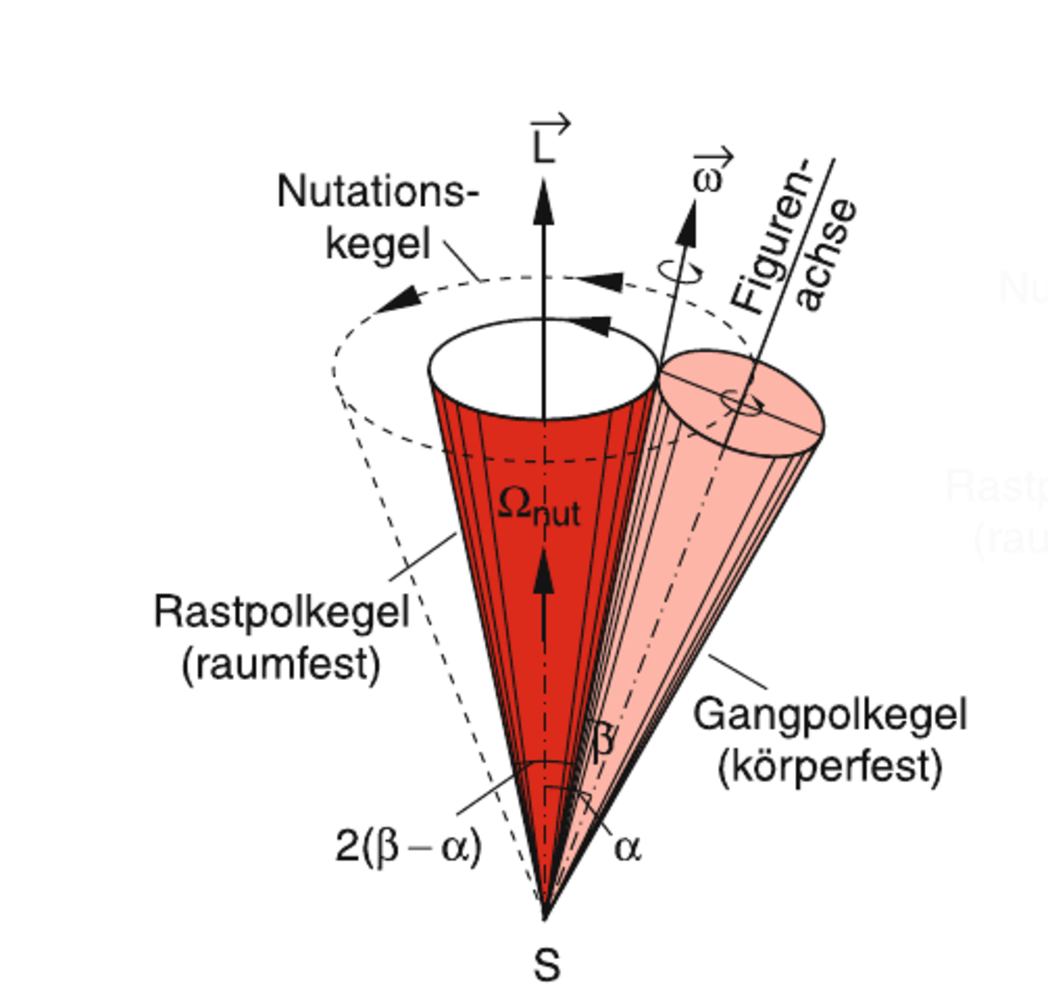
\includegraphics[scale=0.3]{fig/nutationskegel.pdf}
        \caption{Nutationskegel mit Rast- und Gangpolkegel\cite{Demtroeder2017}[s.160f]}
        \label{fig:nutkegel}
    \end{figure}
    
    \section{Versuchsaufbau}
    Es wurde ein auf Kardanrahmen gelagerter Kreisel auf etwa $17Hz$ beschleunigt und mit Hilfe eines Photosensors sowie einem reflektiven Streifen auf dem Kreisel seine Frequenz bestimmt. Nun sollte ein zweiter Sensor auf Höhe des inneren Kardanrahmen angebracht werden um die Frequenz der Nutation zu messen. Damit in dem sonst ruhigen System eine Nutation entsteht, wurde dem Kardanrahmen ein Schlag versetzt.
    \section{Versuchsbeobachtung}
    Nachdem der Kreisel einen Schalg versetzt bekommen hat, führte er eine Taumelbewegung um die Ursprüngliche Drehimpulsachse aus, welche sich nach einigen Sekunden wieder zu wegdämpfte. Hierbei waren die Dauer und Intensität der Nutation abhängig von der momentanen Drehfrequenz des Kreisels. Als Messwerte wurden dann sowohl die Drehfrequenz in $Hz$ als auch die Nutationsfrequenz in $Hz$ aufgenommen.
    \newpage
    \section{Auswertung}
    Wir Tragen die gemessenen Werte in einem Diagramm auf und führen eine lineare Regression durch. Als Fehler wurde die Ungenauigkeit des elektronischen Sensors verwendet, bei welchem wir nur bis zur zweiten stelle nach dem Komma Abgelesen haben. Dies ergibt einen Fehler von $\pm0.01Hz$.
    \begin{figure}[h]
        \centering
        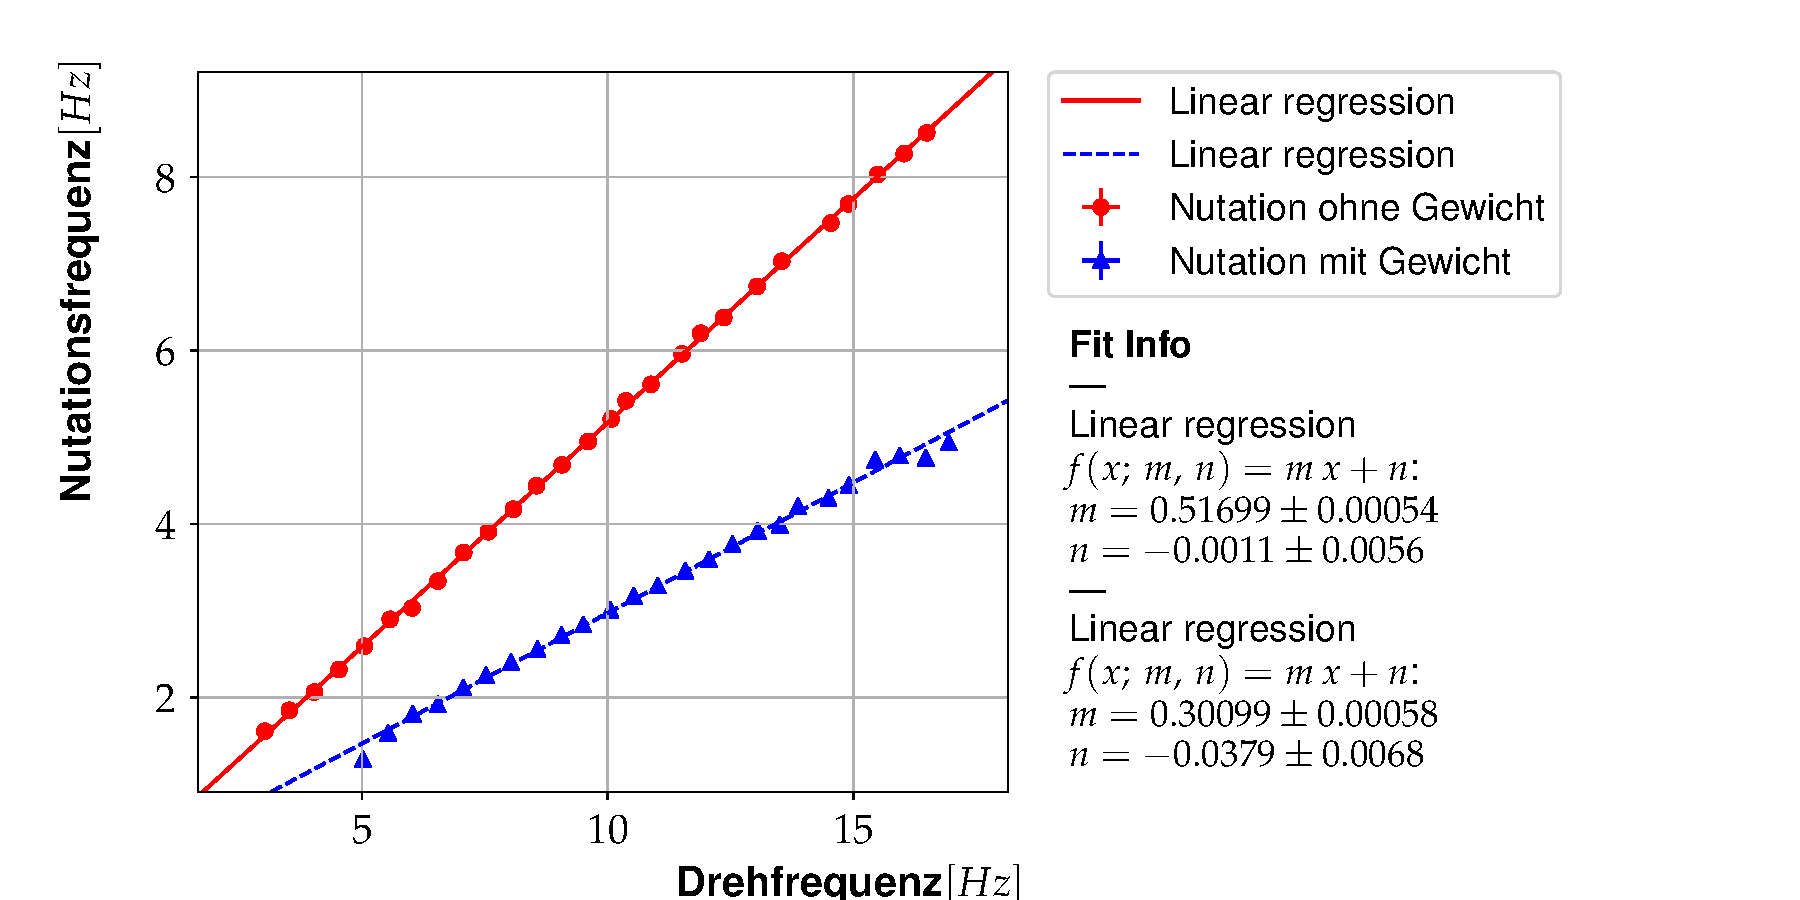
\includegraphics[scale=0.5]{fig/kafe_nutation.pdf}
        \caption{Gemessene Nutatiosfrequenz}
        \label{fig:nuFig}
    \end{figure}
    
    Hierbei erkennt man, dass die Nutationsfrequenz ungefähr der Hälfte der Drehfrequenz entspricht. Mit zwei Zusatzgewichten von je $1$kg, welche am äußeren Kardanrahmen parallel zur Rotationsachse angebracht wurden, erhalten wir ungefähr $\frac{1}{3}$ der unbeschwerten Drehfrequenz. Das zusätzliche Trägheitsmoment, welches durch die Gewichte erzeugt wird berechnet sich wie folgt:
    \begin{equation}\label{eq: theta_g}
        \theta_g=m\left(\frac{d^2}{4}+2l^2\right)
    \end{equation}
    
    
    \chapter{Dämpfung des Kreisel}
    
    \section{Theorie}
    Die Dämpfung des Kreisels wird durch Reibungskräfte bewirkt, derer Natur es zunächst zu bestimmen gilt. Die Experimentresultate legen die Vermutung Nahe, dass es sich um Stokessche Reibung handelt, weswegen diese im Folgenden zur Berechnung verwendet wird. Hierzu geht man von einer Luftreibungskraft am Kreiselmantel aus:
    \begin{align}
        \frac{\d \vec{L}}{\d t} = \vec{M} &= \vec{r} \times \vec{F_s} \\
        \vec{F_s} &= -\gamma \cdot \vec{v} \\
        \vec{v} &= \vec{\omega} \times \vec{r} \\
        \Rightarrow \frac{\d \vec{L}}{\d t} = -\gamma \cdot \vec{r} \times (\vec{w} \times \vec{r}) &= - \gamma r^2\cdot \vec{\omega} \ | \ \mathrm{da\ \vec{r} \cdot \vec{\omega} = 0} \\
        \Rightarrow -\gamma r^2 \cdot \vec{\omega} &= \frac{\d L}{\d t} = \theta \cdot \frac{\d \vec{\omega}}{\d t} \\
        \Rightarrow \vec{\omega}(t) = \vec{\omega_0} \cdot \exp{\left(-\frac{\gamma r^2}{\theta} t\right)} &= \vec{\omega_0} \cdot \exp{\left(-\frac{\gamma}{m} t\right)}
    \end{align}
    Demnach sollte bei alleiniger Wirkung der Luftreibung die Frequenz des Kreisels einen exponentiellen Abfall beschreiben. Dies lässt sich auch anhand unserer Messdaten erkennen:
    \begin{figure}[H]
    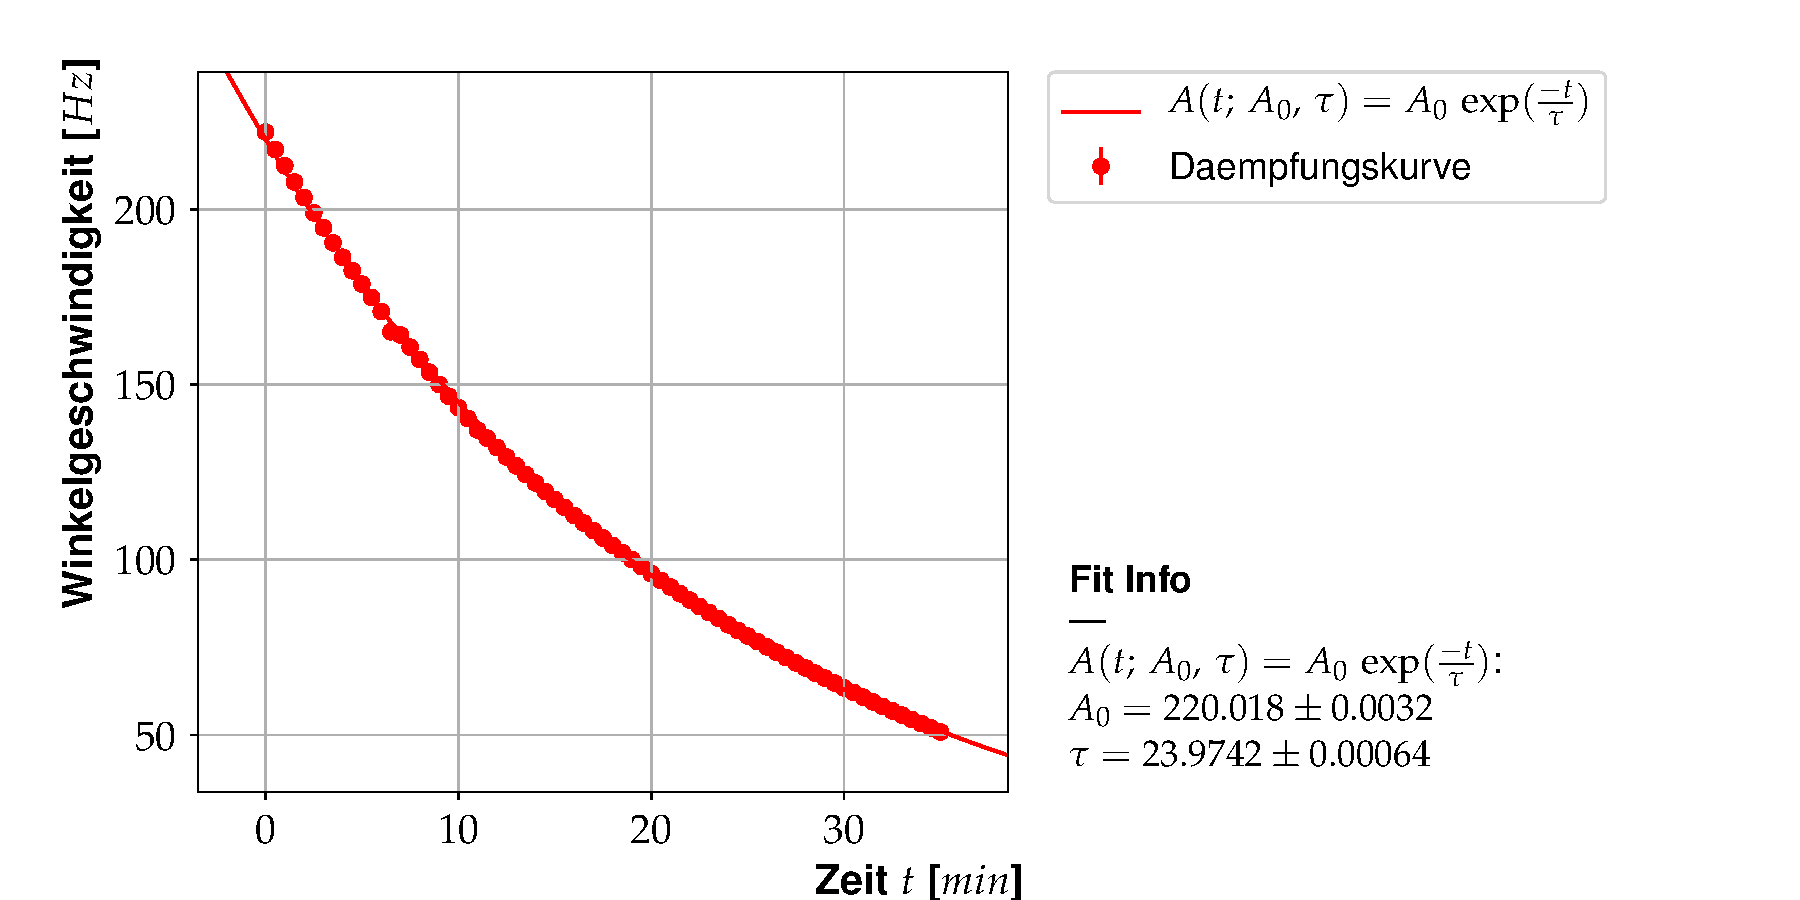
\includegraphics[scale=0.45]{fig/kafe_daempfungskurve.pdf}
    \end{figure}
    Da andere Arten von Reibung zu einer Abweichung vom exponentiellen Abfall führen würden, lassen sich in unserem Messbereich die Wirkungen derer vernachlässigen. Darüber hinaus ließe sich nun durch einen zweiten Kreisel bekannten Gewichts und gleicher Ausmaße (Länge) das Gewicht des Unseren bestimmen, durch Vergleich der Fitparameter $\tau$.
    
    \chapter{Wirken von Drehmomenten}
    
    \section{Theorie}
    Das Wirken von Drehmomenten, in unserem Fall der Schwerkraft, führt am Kreisel zu Präzessionsbewegungen. Diese lassen sich durch ihre unintuitive Richtung charakterisieren, welche senkrecht auf die eigentlich wirkende Kraft steht. Wie diese aus dem Drehimpuls resultiert wird im Folgenden gezeigt:
    \begin{align}\label{eq:praezission}
        \frac{\d \vec{L}}{\d t} = \vec{M} &= (\vec{r} \times \vec{F}) = -mg(\vec{r} \times \vec{e}_z) \\
        \Leftrightarrow \frac{\d \omega_K}{\d t} &= -\frac{mg}{\theta}(\vec{r} \times \vec{e}_z) \\
        \mathrm{mit\ } \vec{\omega}_K=|\omega_K|\cdot \vec{e}_r \ \Big\vert \Rightarrow -\frac{mgr}{\theta}(\vec{e}_r \times \vec{e}_z) &= -\frac{mgr}{\theta} \sin(\theta) \vec{e}_{§} = -\omega_K \cdot \dot\phi\sin(\theta)\vec{e}_§ \\
        \Leftrightarrow \frac{mgr}{\theta} &= \omega_K \dot\phi \\
        \mathrm{Pr"azessionsfrequenz}\hat{=} \dot\phi = \omega_p &= \frac{mgr}{\theta \cdot \omega_K}
    \end{align}
    \section{Experiment}
    Man kann nun die Umlaufzeiten der Pr"azession messen und gegen die Drehfrequenz auftragen, dies führt zu folgendem $\frac{1}{\omega_p}-\omega_K-$Diagramm, welches mittels einer Ursprungsgerade gefittet werden kann. Ihre Steigung $m= \frac{\theta \cdot 4 \pi^2}{mgr}$ bestimmt sich gemäß der Gleichung $g(f_k)=\frac{1}{f_p}=\frac{\theta \cdot 4 \pi^2}{mgr}f_K$ mit $2 \pi f_p = \omega_p \mathrm{\ und\ } 2\pi f_K = \omega_K$. \\
    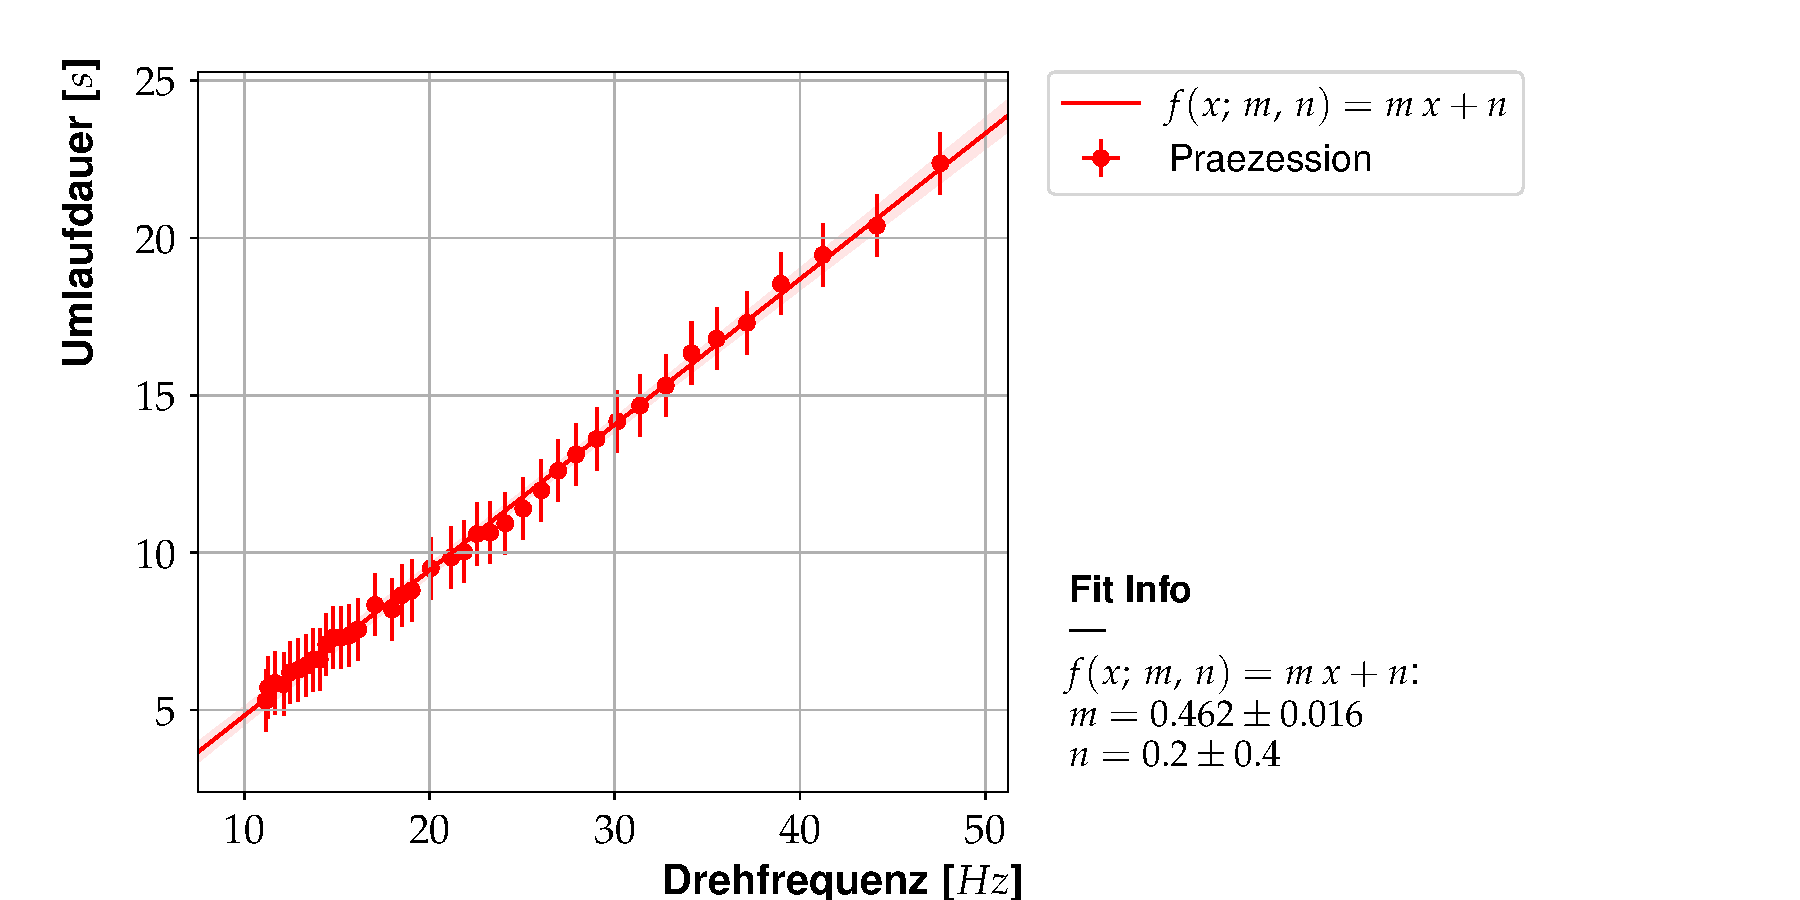
\includegraphics[scale=0.5]{fig/kafe_praezession.pdf}
    \chapter{Hauptträgheitsmomente}
    
    \section{Theorie}
    Zur Berechnung der Hauptträgheitsmomente werden die Gemessenen Präzessions- und Nutationsfrequnezen des symmetrischenKreisels, unter Berücksichtigung der zusätzlichen Trägheitsmomente der Kardanrahmen, verwendet. Daraus wird dann eine Schätzung der Masse des Rotors formuliert.
    
    Nun gilt laut \eqref{eq:3.8} und der Annahme kleiner Öffnungswinkel der Kegel:
    \begin{equation}\label{eq:tbd}
        \omega_{\perp}=\frac{\theta_c}{\sqrt{A\cdot B}}\omega
    \end{equation}
    Dies bestätigt auch die Formel aus dem Vorbereitungsmaterial und weiterhin lässt sich sagen \cite{PhyPra1}[vgl. S.9f]: 
    \begin{align}
        A&=\theta_{a}^{Kreisel}+\theta_a^{Innenkardan}+\theta_a^{Au"senkardan}\\
        \nonumber B&=\theta_b^{Kreisel}+\theta_b^{Innenkardan}
    \end{align}
    Verwendet man nun die Formel \eqref{eq:praezission} aus Aufgabe 5, so erhält man für das Hauptträgheitsmoment um die Achse $c$ : 
    \begin{equation}
        \theta_c=\frac{mgr}{\omega_p\omega_k}
    \end{equation}
    wobei $m$ der Masse des Stabs entspricht und $r$ der Abstand vom Schwerpunkt des Kreisels zum Schwerpunkt des Stabs ist. Die beiden Winkelfrequenzen erhalten wir aus unseren Messwerten:
    \begin{align}
    \omega_p&=2\pi f_p\\
    \nonumber\omega_k&=2\pi f_k
    \end{align}
    Aus der Steigung der Fit gerade lässt sich dann die Formel wie folg schreiben:
    \begin{align}
    \frac{1}{\omega_p}&=\frac{\theta\omega_k}{mgr}\\
    \nonumber\frac{1}{2\pif_p}&=\frac{\theta2\pi f_k}{mgr}\\
    \nonumber\frac{1}{f_p}&=\frac{4\theta\pi^2f_k}{mgr}\\
        g(f_k)&=\frac{1}{f_p}=m\cdot f_k\\
        \nonumber\Rightarrow m&=0.462=\frac{4\pi^2\theta}{mgr}
    \end{align}
    somit erhalten wir für $\theta_c = \frac{mgr}{4\pi^2 m_{präzession}}$
    mit den gemessenen Werten:
    \begin{align}
        \theta_c&=\frac{(r_{Innenrahmen}+r_{Schwerpunkt,Stab})\cdot m_{Stab\cdot g}}{4\pi^2\cdot m_{(steigung),p}}\\
        \theta_c&=\frac{0.33kg\cdot(0.109m+0.178m)\cdot 9.81\frac{m}{s^2}}{4\pi^2\cdot 2.06 s^{-2}}\\
        \theta_c&=0,0113 kgm^2
    \end{align}
    
    Nun verwenden wir die ermittelten Steigungen und den Trägheitsmoment der Zusatzgewichte aus Aufgabe 3 um A und B zu bestimmen:
    \begin{align}
        A&=\frac{\theta_G}{\left(\frac{m_{nut}^{ohne}}{m_{nut}^{mit}}\right)^2-1}\\\theta_g&=1kg\left(\frac{(0.04m)^2}{4}+2*(0.149m)^2\right)=0.0448kgm^2\\A&=\frac{0.0488kgm^2}{\frac{0.516^2}{0.309^2}-1}=0.0272kgm^2
    \end{align}
    Daraus folg nun auch $B$:
    \begin{align}
    B&=\frac{\theta_c^2}{m_{nut}^{(ohne)2}\cdot A}\\
    B&=\frac{(0.0113kgm^2)2}{(0.516^2)\cdot 0.0272kgm^2=0.0177kgm^2}
    \end{align}

\begin{table}[h]
\centering
\begin{tabular}{|l|l|l|}
\hline
$\theta_c$ & 0.0113 & $kgm^2$ \\ \hline
A          & 0.0272 & $kgm^2$ \\ \hline
B          & 0.0177  & $kgm^2$ \\ \hline
\end{tabular}
\end{table}

Zur Abschätzung der Rotormasse verwenden wir die Formel des Trägheitsmoments für einen Zylinder:
\begin{align}
    \theta&=\frac{1}{2}mr^2\\
    \theta_c&=\frac{1}{2}m\left(\frac{d_{zylinder}}{2}\right)^2\\
    m&=\frac{8\theta_c}{d_{zylinder}^2}\\
    m&=\frac{8\cdot 0.0113kgm^2}{(0.135m)^2}=4.96kg
\end{align}

Somit wäre die geschätzte Masse des Rotos $5kg$.
    
    \chapter{Kreisel im beschleunigten Bezugssystem}
    
    \section{Theorie}
    Der vorgeführte Kreisel, auch "Kreiselkompass" \ genannt, ist mithilfe von Federn an die Horizontalebene gebunden. Diese Bindung beschränkt seine Freiheitsgrade zur Ausrichtung auf zwei, nämlich kann der Drehimpuls nun nur in der Horizontalebene kräftefrei liegen.
    \begin{wrapfigure}{l}{0.5\textwidth}
    \centering
    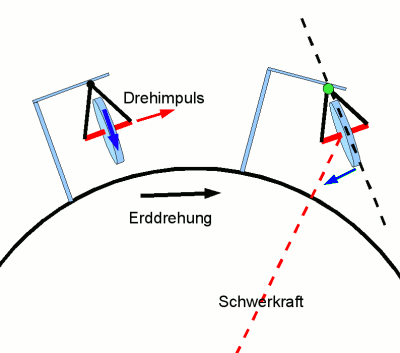
\includegraphics[scale=0.5]{fig/kreisel.png}\footnote{https://wissenstexte.de/physik/kreisel.png}
    \caption{Funktionsweise des Kreiselkompass}
    \label{F1}
    \end{wrapfigure}
    Liegt der Drehimpuls auch nur infinitesimal außerhalb der Horizontalebene, wirken wie in Abb. \ref{F1} zu sehen, Drehmomente auf die Aufhängung des Kreisels, welche als zeitliche Ableitung des Drehimpulses des Gesamtsystems auch auf selbigen wirken. Dies führt zu einer Verschiebung des Drehimpulses ''in Richtung des Nordpols'' wobei dieser hierbei rein durch die Rotationsbewegung der Erde, relativ zum Kreisel, definiert ist. Dementsprechend richtet sich der Kreisel bei gleicher Eigenrotation aber umgekehrter Erdrotation auch zum Südpol statt dem Nordpol aus, wobei selbiges für normale Erdrotation aber umgekehrter Kreiselrotation gilt. Allgemein lässt sich sagen, das der Kreiselkompass sich immer zum Schnnittpunkt seiner Horizontalebene und dem Drehimpuls seiner Basis ausrichtet, allerdings muss seine Position hierzu auf ihr festgesetzt sein. Bewegt sich der Kreisel orthogonal zur Erdrotation, d.h. auf einem Breitengrad, simuliert dies lediglich einen vergrößerten Drehimpuls, verändert die Richtung des Kompass allerdings nicht. Ganz anders sieht es jedoch bei einer Bewegung entlang eines Meridians aus, d.h. sodass $\vec{v}\cdot \vec{L} \not= 0$. In diesem Fall weist die Kompassrichtung Abweichungen auf, welche aufgrund der zusätzlichen Drehmomente auftreten und von der Geschwindigkeit entlang des Meridians abhängen. Aus diesem Grund wird der Kreiselkompass auch tendenziell eher auf langsamen Fortbewegungsmitteln wie Schiffen genutzt, nicht aber auf Flugzeugen, da durch deren hohe Geschwindigkeiten zu starke Abweichungen auftreten können.
\chapter{Fehleranalyse}
Als Fehler sind in unseren Versuchsreihen größtenteils die Sensoren an den Schwanenhälsen zu sehen, da diese nicht konsistent die richtigen Frequenzen angezeigt haben, sondern zwischen sehr hochzahligen Frequenzen und der tatsächlichen Frequenz der Messung schwanken. Somit war es schierig die richtige Frequenz der Nutation zu bestimmen, als auch der Drehfrequenz in sehr hohen und niedrigen Bereichen. Bei der Dämpfung hatten wir auf Grund eines gut laufenden Kreisels keinen linearen Abfall der Funktionswerte gegen Ende der Messung, sondern nur einen exponentialen Abfall
%\listoffigures    
\bibliography{verweise.bib}
\bibliographystyle{plain}
\end{document}
